\chapter{Evaluation}

In this chapter we describe how we utilized our system to run our experiments. We provide a quantitative analysis of the data that we gathered and the comparison between the different experiment settings.

\section{Objectives}

We hypothesize that we are able to enhance the classification accuracy of our image classifier using synthetic data for training. We examine multiple ratios of synthetic to real images for training. Moreover, we run our experiments on multiple CNN architectures and fine-tune them accordingly.


\section{Methodology}

Our methodology is divided into 2 main parts: Image Collection and Training the Image Classifier. Image Collection is concerned with the real and synthetic images, and how they're collected from small parts and their corresponding 3D models. Training the Image Classifier revolves around utilizing the collected images to maximize the classification accuracy of the image classifier.

\subsection{Image Collection}

During image collection, we strive to create a synthetic dataset that has a high degree of photo-realism. Simultaniously, we want to create 3D models as fast as possible to decrease the timing of the whole workflow. To achieve this balance, we aim to create an environment that is easy to model on 3D software. We attempt to eliminate light reflections and shadows and reduce the overall complexity of the scene.

\subsubsection{Small Parts and their corresponding 3D Models}
We first choose a small part that we wish for our image classifier to recognize. We then download the corresponding 3D model by searching the Traceparts website\footnote{https://www.traceparts.com} for the small part's code name.
% TODO: Add real and synthetic images of all of our 6 classes

\subsubsection{Collecting Real Images}
We place the chosen small model on a horizontal plane and place a light source underneath. We choose a plain, white, semi-transparent plane as a background to disperse the light source coming from underneath, and distribute the light evenly accross the plane. We place the light source beneath the plane, rather than above, to eliminate any shadow that the small parts might cast. Moreover the dispersed back light provides a lighting source without casting a direct light on the objects, which might cause glare on the small part's reflective surface.

Next, we place a an iPhone over the plane, such that the small object is fully within the viewfield of the iPhone's camera. A wooden setup places the iPhone 133 mm over the plane as shown in figure [\ref{fig:RealSetup}].

Afterwards, we rotate and change the position of the small part randomly, while maintaining that the small part is fully within the viewfield of the camera. We use the iPhone's camera to take a picture of the small part. We repeat this step until we obtain the desired number of real images.

Lastly, we resize the raw real images taken by the iPhone camera to conform with the height and width required by the image classifier.

\subsubsection{Generating Synthetic Images}
We start by creating the synthetic scene in the Rhinoceros 3D modeling software. First, we take a picture of the real horizontal plane and use it as a background for our synthetic scene. We then place a synthetic lighting source underneath the plane to mimic the lighting effect of the real environment. Next, we place the 3D model on the horizontal plane of the environment.

Next, we generate a python script that uses the Rhinoceros library to manipulate 3D objects in the Rhinoceros software. The python script is the controller for the synthetic data genertor. The synthetic data generator obtains the rotation and translation ranges of the 3D model. It also specifies how many images are to be generated. For each new image, the script generates a random rotation and translation value from within the defined ranges. It then applies those transformation to the 3D model and renders a new 2D synthetic image.

\begin{figure}[H]
\centering
  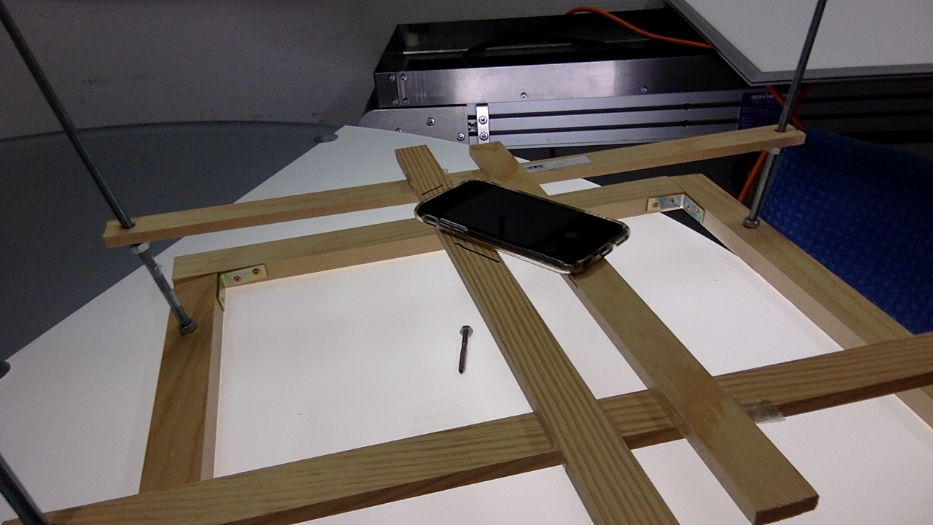
\includegraphics[width=0.95\textwidth]{real_setup}
\caption{Set up of generating real images. An iPhone is placed on a wooden setup over a horizontal, backlit glass table with opal foils. The small part rests on the table within the viewfield of the iPhone camera.}
\label{fig:RealSetup}
\end{figure}

\begin{figure}[H]
\centering
  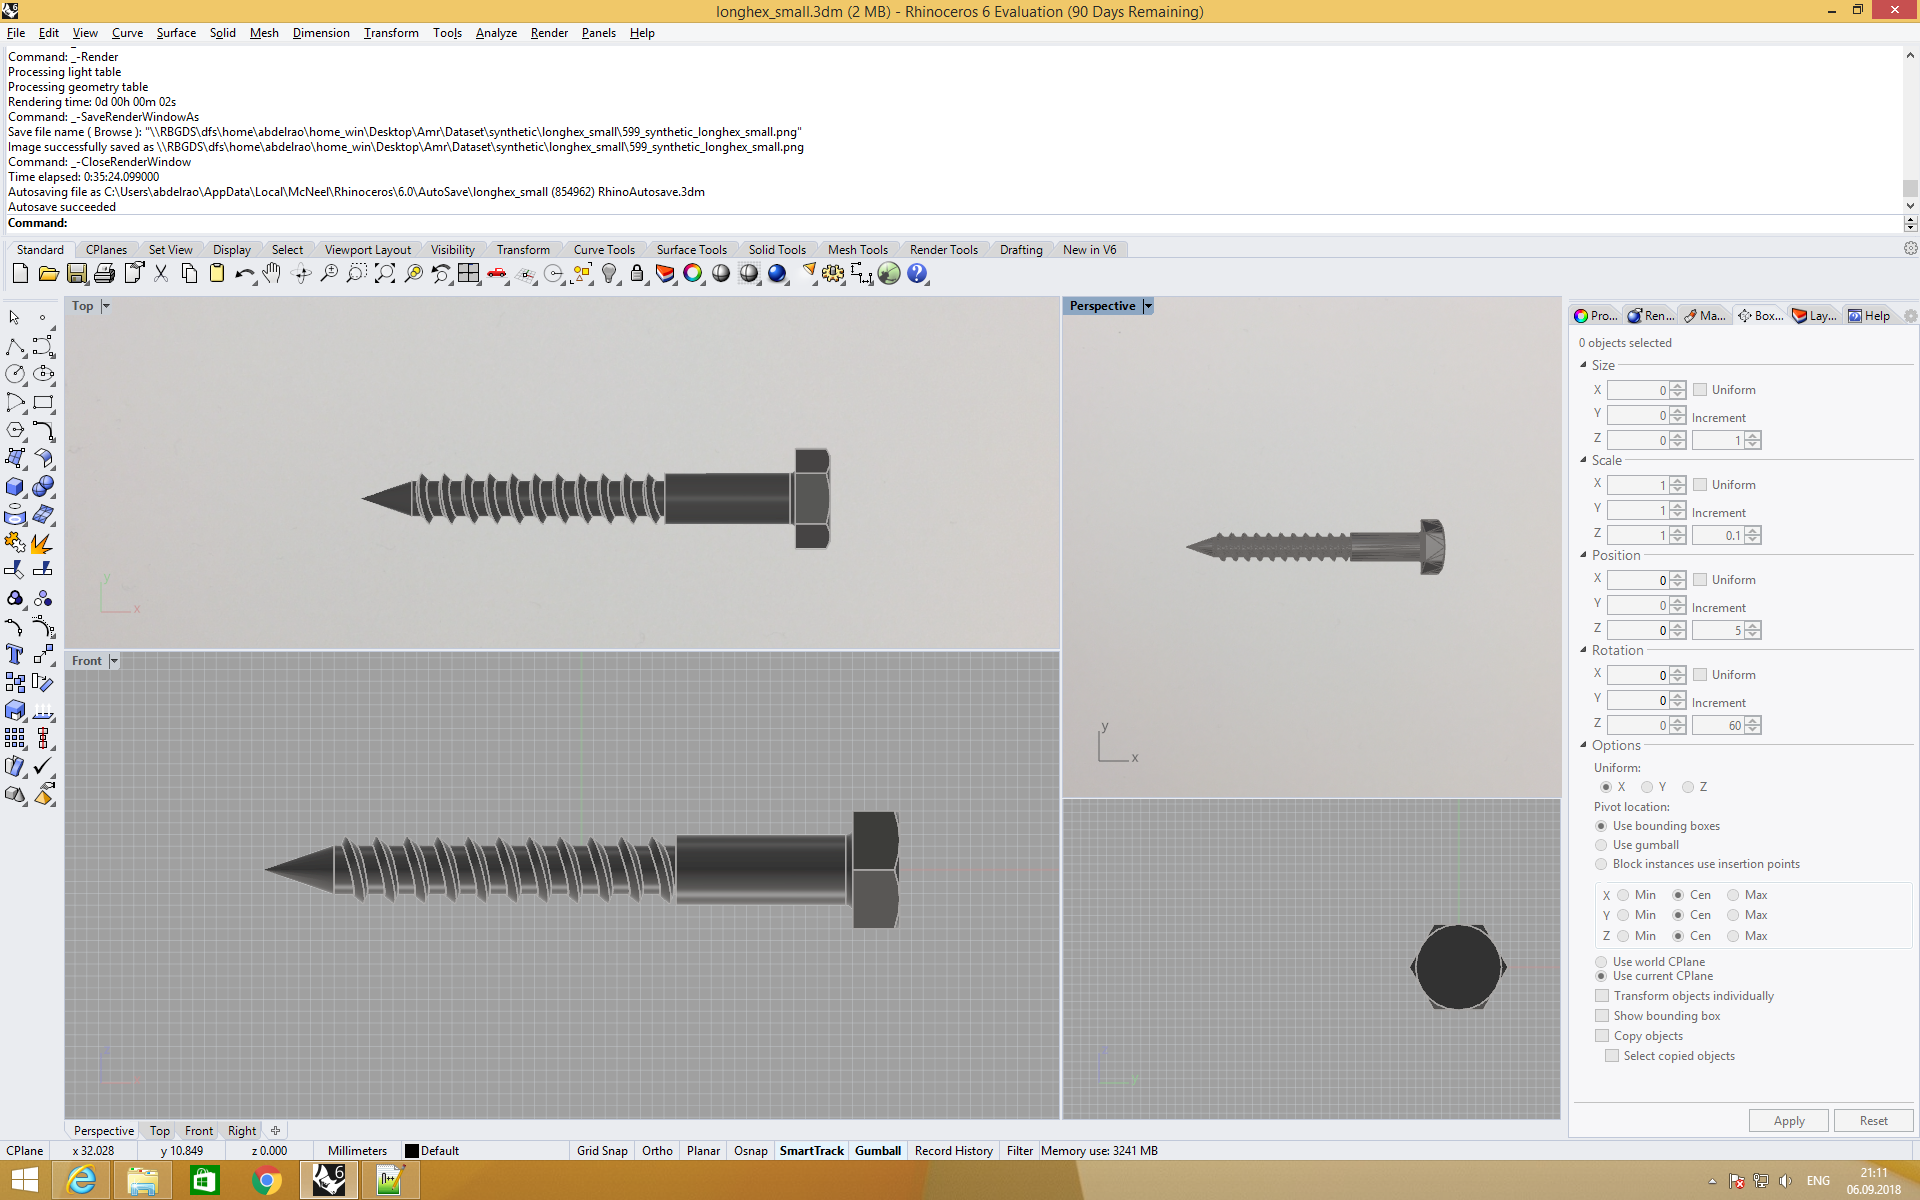
\includegraphics[width=0.95\textwidth]{rhino_screenshot}
\caption{Synthetic scene in Rhino. The 3D model rests horizontally on a backlit plane to mimic the environment of the real setup. Sections (a) and (b) of the image depict the top view of the scene.}
\label{fig:RhinoScreenshot}
\end{figure}

\subsubsection{Dataset}
The real images generated from the small part and the synthetic images generated from the corresponding 3D model are transfered to the Training Machine where they are placed in the dataset folder.

\subsection{Training the Image Classifier}
The image classifier uses the images that we generate to train a convolutional neural network model to classify images of our small parts.

\subsubsection{Data Split Generator}
We first split our images into a training set, a validation set and a testing set. Moreover, we determine the number of synthetic images vs the number of real images in our training set. The data split generator organizes the images in folder named after the label of their respective small part. The images are organized as shown in figure [\ref{fig:FS}].

We compare the performance of 5 different ratios of synthetically enhanced training sets. Table [\ref{tab:DS}] describe our different data splits, detailing the number of images per class for each split. We generate a fully synthetic training set, a 2.5\% real training set, a 5\% real training set, a 10\% real training set, and a fully real training set. 

\begin{table}[H]
\centering
\begin{tabular}{|l|l|l|l|l|l|}
\hline
\textbf{Data Split} & \multicolumn{1}{c|}{\textbf{\begin{tabular}[c]{@{}c@{}}Training\\ (Synthetic)\end{tabular}}} & \multicolumn{1}{c|}{\textbf{\begin{tabular}[c]{@{}c@{}}Training\\ (Real)\end{tabular}}} & \multicolumn{1}{c|}{\textbf{\begin{tabular}[c]{@{}c@{}}Training\\ (Total)\end{tabular}}} & \multicolumn{1}{c|}{\textbf{Validation}} & \multicolumn{1}{c|}{\textbf{Testing}} \\ \hline
\textbf{0\%} & 600 & 0 & 600 & 100 & 150 \\ \hline
\textbf{2.5\%} & 585 & 15 & 600 & 100 & 135 \\ \hline
\textbf{5\%} & 570 & 30 & 600 & 100 & 120 \\ \hline
\textbf{10\%} & 540 & 60 & 600 & 100 & 90 \\ \hline
\textbf{100\%} & 0 & 150 & 150 & 50 & 50 \\ \hline
\end{tabular}
\caption{Each column details the number of images per class for the specified data split.}
\label{tab:DS}
\end{table}

\subsubsection{CNN Model}
The convolutional neural network model refers to the CNN architecture, the used optimizer and their respective hyperparameters. For each data split, we attempt to use the VGG16 and the VGG19 architecture \cite{simonyan2014very}. Moreover, we attempt to use the Stochastic Gradient Descent (SGD) optimizer \cite{bottou2018optimization} and the Adam optimizer \cite{kingma2014adam}. We leverage the power of transfer learning by using CNN models that are pre-trained on the imagenet dataset \cite{deng2009imagenet}. Furthermore, we tweak our CNN models to train and evaluate images of size 500px by 500px.

\subsubsection{Hyperparameter Tuning}
For each data split, we fine tune the hyperparameters of the CNN model to maximize the classification accuracy of the output. Below is a list of hyperparameters that are optimized in the fine-tuning phase.

\begin{itemize}
  \item \textbf{Number of Frozen Layers}: Our CNN models are pre-trained on the imagenet dataset, which means that each layer is preloaded with optimized weights. During training, we freeze some of the early layers to preserve these optimized weights, ie—the frozen layers are set to be untrainable. We optimize our classification accuracy by fine tuning the number of frozen layers.
  \item \textbf{Batch Size}: During training, our CNN model processes the training set in batches. The batch size tells the CNN model how many training images are to be processes similtaneously.
  \item \textbf{Number of Epochs}: An epoch is when the entire training set has been passed through the CNN. Due to the iterative nature of the training process, a CNN has to train for multiple epochs until it reaches maximum classification accuracy.
  \item \textbf{Optimizer Learning Rate}: Learning rate is the rate of change of the network parameter during training. If the learning rate is too small, the weights will take a longer amount of time until they are optimized. If the larning rate is too big, the optimizer might jump over the optimum parameter values, and never actually reach the optimum values.
\end{itemize}

\section{Results}

Tables [\ref{tab:vgg16-results}] and [\ref{tab:vgg19-results}] provide the resulting class-wise classification accuracies of training a VGG16 network and a VGG19 network respectively. The displayed results are reached after fine-tuning the hyperparameters described in the previous section. The provided classification accuracy is the result of evaluating each CNN model using the respective testing set.

\begin{table}[H]
\centering
\begin{tabular}{|l|c|c|c|c|c|c|c|}
\hline
\textbf{\begin{tabular}[c]{@{}l@{}}Data\\ Split\end{tabular}} & \textbf{\begin{tabular}[c]{@{}c@{}}Flat\\ Head\end{tabular}} & \textbf{\begin{tabular}[c]{@{}c@{}}Hex\\ Large\end{tabular}} & \textbf{\begin{tabular}[c]{@{}c@{}}Hex\\ Small\end{tabular}} & \textbf{\begin{tabular}[c]{@{}c@{}}Long-\\ hex\\ Large\end{tabular}} & \textbf{\begin{tabular}[c]{@{}c@{}}Mush-\\ room\\ Large\end{tabular}} & \textbf{\begin{tabular}[c]{@{}c@{}}Mush-\\ room\\ Small\end{tabular}} & \textbf{Total} \\ \hline
\textbf{0\%} & 99.333 & 48.000 & 98.667 & 96.667 & 80.667 & 78.000 & \textbf{83.556} \\ \hline
\textbf{2.5\%} & 100.00 & 79.259 & 99.259 & 99.259 & 83.704 & 80.741 & \textbf{90.370} \\ \hline
\textbf{5\%} & 100.00 & 95.833 & 100.00 & 97.500 & 90.833 & 75.833 & \textbf{93.333} \\ \hline
\textbf{10\%} & 100.00 & 94.444 & 98.889 & 100.00 & 98.889 & 90.000 & \textbf{97.037} \\ \hline
\textbf{100\%} & 100.00 & 98.000 & 100.00 & 98.000 & 78.000 & 92.000 & \textbf{94.333} \\ \hline
\end{tabular}
\caption{Class-wise classification accuracy of a VGG16 network trained on different ratios of synthetic data.}
\label{tab:vgg16-results}
\end{table}


\begin{table}[H]
\centering
\begin{tabular}{|l|c|c|c|c|c|c|c|}
\hline
\textbf{\begin{tabular}[c]{@{}l@{}}Data\\ Split\end{tabular}} & \textbf{\begin{tabular}[c]{@{}c@{}}Flat\\ Head\end{tabular}} & \textbf{\begin{tabular}[c]{@{}c@{}}Hex\\ Large\end{tabular}} & \textbf{\begin{tabular}[c]{@{}c@{}}Hex\\ Small\end{tabular}} & \textbf{\begin{tabular}[c]{@{}c@{}}Long-\\ hex\\ Large\end{tabular}} & \textbf{\begin{tabular}[c]{@{}c@{}}Mush-\\ room\\ Large\end{tabular}} & \textbf{\begin{tabular}[c]{@{}c@{}}Mush-\\ room\\ Small\end{tabular}} & \textbf{Total} \\ \hline
\textbf{0\%} & 100.00 & 81.333 & 88.667 & 92.000 & 98.667 & 52.667 & \textbf{85.556} \\ \hline
\textbf{2.5\%} & 100.00 & 100.00 & 86.667 & 99.259 & 99.259 & 90.370 & \textbf{95.926} \\ \hline
\textbf{5\%} & 100.00 & 100.00 & 96.667 & 98.333 & 100.00 & 88.333 & \textbf{97.222} \\ \hline
\textbf{10\%} & 100.00 & 90.000 & 96.667 & 98.889 & 98.889 & 96.667 & \textbf{96.852} \\ \hline
\textbf{100\%} & 100.00 & 92.000 & 98.000 & 96.000 & 78.000 & 90.000 & \textbf{92.333} \\ \hline
\end{tabular}
\caption{Class-wise classification accuracy of a VGG19 network trained on different ratios of synthetic data.}
\label{tab:vgg19-results}
\end{table}

\section{Findings}

In our experiments, synthetic data has been found to enhance the classification accuracy of both the VGG16 and the VGG19 models. We note that using the purely real datasets, the VGG16 network reached a classification accuracy of 94.333\%, while using the 10\% real data training set resulted in an accuracy of 97.037\%. Moreover, the VGG19 network achieved an accuracy of 92.333\% using only real data, compared to an accuracy of 97.222\% as a result of using the 5\% real data training set.

Furthermore, we notice that the small parts with the highest class-wise accuracy are \textit{Flat Head} and \textit{Longhex Large}. Compared to their counterparts, those two small parts have a unique aesthetic. Hex Large and Hex small look similar, and the same goes for Mushroom Large and Mushroom Small.

\section{Limitations}

Our system is dependant on having access to the 3D model of the small parts in order to generate synthetic images. Moreover, the model's classification accuracy is dependant on the shapes of the small parts. As observed in the previous section, the class-wise accuracy for an object that is similar to other objects in the dataset is lower than an object that is aesthetically unique.